\documentclass[12pt,a4paper,twoside]{book}
\usepackage{a4wide}                     % Iets meer tekst op een bladzijde
\usepackage[dutch,english]{babel}       % Voor nederlandstalige hyphenatie (woordsplitsing)
\usepackage{amsmath}                    % Uitgebreide wiskundige mogelijkheden
\usepackage{amssymb}                    % Voor speciale symbolen zoals de verzameling Z, R...
\usepackage{url}                        % Om url's te verwerken
\usepackage{graphicx}                   % Om figuren te kunnen verwerken
\usepackage[small,bf,hang]{caption}    % Om de captions wat te verbeteren
\usepackage{xspace}                     % Magische spaties na een commando
\usepackage[latin1]{inputenc}           % Om niet ascii karakters rechtstreeks te kunnen typen
\usepackage{float}                      % Om nieuwe float environments aan te maken. Ook optie H!
\usepackage{flafter}                    % Opdat floats niet zouden voorsteken
\usepackage{listings}                   % Voor het weergeven van letterlijke text en codelistings
\usepackage{marvosym}                   % Om het euro symbool te krijgen
\usepackage{textcomp}                   % Voor onder andere graden celsius
\usepackage{fancyhdr}                   % Voor fancy headers en footers.
\usepackage{graphics}			% Om figuren te verwerken.
\usepackage[nottoc]{tocbibind} % Bibliografie in ToC; zie tocbibind.dvi
%\usepackage{pstricks}
\usepackage{longtable}
\usepackage{pdfpages}  % pdf pagina's importeren
%\usepackage[plainpages=false]{hyperref}    % Om hyperlinks te hebben in het pdfdocument.
\usepackage[dutch]{babel} %for dutch-like character
\usepackage{titletoc}%
\usepackage{titlesec}%to control chapter title format

%settings for the table of contents
\titlecontents{chapter}% <section-type>
  [0pt]% <left>
  {\bfseries}% <above-code>
  {\chaptername\ \thecontentslabel:\quad}% <numbered-entry-format>
  {}% <numberless-entry-format>
  {\hfill\contentspage}% <filler-page-format>

\newcommand{\npar}{\par \vspace{2.3ex plus 0.3ex minus 0.3ex} \noindent}	% Om witruimte te krijgen tussen paragrafen
\graphicspath{{figures/}}               % De plaats waar latex zijn figuren gaat halen.


\newcommand{\command}[1]{\lstinline[basicstyle=\tt]{#1}\xspace} %Voor commando's
\hyphenation{he-den-daag-se ap-pa-ra-tuur Meet-re-sul-ta-ten hand-o-ver-tijd ho-ge-snel-heids-trein}


%setting toc entries for the box
\newcommand*\TocHeadingBoxA
{\noindent\parbox[t]{\textwidth}{\bf \Large{Box A: \hspace*{1.35cm} Title of Box A \hfill \pageref{boxa-pagenb}}}\par
 \global\let\TocHeadingBoxA\empty }


%\titleformat{\chapter}{\tiny}{\chaptername \large{\thechapter}}{}

% Het bibliografisch opmaak bestand.
\bibliographystyle{unsrt}
%\bibliographystyle{bibliodutch}
%\bibpunct{[}{]}{,}{n}{,}{,}

\renewcommand{\chaptermark}[1]{\markright{\uppercase{#1}}}
\renewcommand{\sectionmark}[1]{\markright{\thesection~#1}}

\newcommand{\headerfmt}[1]{\textsl{\textsf{#1}}}
\newcommand{\headerfmtpage}[1]{\uppercase{#1}}

%\lhead[\thechapter]{}
%\rhead[]{\chaptername \thechapter}


%\fancyhead[LE,RO]{\headerfmtpage{\thepage}}
%\fancyhead[LO]{\headerfmt{\rightmark}}
%\fancyhead[R]{\headerfmt{\leftmark}}
%\renewcommand{\headrulewidth}{0.5pt}
%\renewcommand{\footrulewidth}{0pt}

\fancypagestyle{plain}{ % eerste bladzijde van een hoofdstuk
  \fancyhf{}
  \fancyhead[LO]{\textsc{\chaptername~ \thechapter}}
  \fancyhead[RE]{\headerfmtpage{\rightmark}}
  \fancyfoot[LO]{\thepage}
  \fancyfoot[RE]{\thepage}
  %\fancyhead[LO]{\headerfmt{\rightmark}}
  %\fancyhead[RE]{\headerfmt{\thechapter}}
  %\fancyhead[LO]{\headerfmt{\rightmark}}
  %\fancyhead[R]{\headerfmt{\leftmark}}
  \renewcommand{\headrulewidth}{0.5pt}
  \renewcommand{\footrulewidth}{0pt}
}

\renewcommand{\lstlistoflistings}{\begingroup
   \tocfile{\lstlistlistingname}{lol}
\endgroup}


% anderhalve interlinie (opm: titelblad gaat uit van 1.5)
\renewcommand{\baselinestretch}{1.5}


%\hypersetup{
%    pdfauthor = {DVL},
%    pdftitle = {Cooperative breeding},
%    pdfsubject = {PhD from DVL}
%}

\begin{document}
\nocite{*}
%\selectlanguage{dutch}
\renewcommand\lstlistlistingname{Lijst van codefragmenten}
\renewcommand\lstlistingname{Codefragment}

\pagenumbering{gobble} %to remove page numbering
%first two pages of the book

\Large{The title of the thesis}

\newpage

\vspace{6cm}



\includegraphics[height=1cm]{fwo_logo}

\paragraph*{}
Funding acknoledgements 

\paragraph*{}
Nedlandse titel

\paragraph*{}

Layout and figures:

\pagestyle{empty}


%\input{s-titel}

% lege pagina (!!)
%\newpage
%\vfil\null
%\newpage


% titelblad (!!)
\thispagestyle{empty}
%  Titelblad

% Opmerking: gaat uit van een \baselinestretch waarde van 1.5 (die moet
% ingesteld worden voor het begin van de document environment)

\begin{titlepage}

%\setlength{\hoffset}{-1in}
%\setlength{\voffset}{-1in}
%\setlength{\topmargin}{1.5cm}
%\setlength{\headheight}{0.5cm}
%\setlength{\headsep}{1cm}
%\setlength{\oddsidemargin}{3cm}
%\setlength{\evensidemargin}{3cm}
%\setlength{\footskip}{1.5cm}
%\enlargethispage{1cm}
% \textwidth en \textheight hier aanpassen blijkt niet te werken

\fontsize{12pt}{14pt}
\selectfont

\begin{center}


\textsc{Gent Universiteit}

\vspace*{\fill}

{\huge \bf Title of the thesis}

\vspace*{\fill}

\textsc{Proefschrift}

\vspace*{\fill}

door

\vspace*{\fill}

DVL\\

born ...

\end{center}

\clearpage

\begin{tabular}{ll}
 Promoters: & LL \\
 Copromotor: & Someone else \\
 Paranifs: & Someone else
\end{tabular}


\end{titlepage}

\thispagestyle{empty}

% geen paginanummering tot we aan de inhoudsopgave komen
\thispagestyle{empty}
\pagenumbering{roman}
\frontmatter
\tableofcontents

\pagenumbering{arabic}
\mainmatter
\setlength{\headheight}{15pt}
\pagestyle{plain}







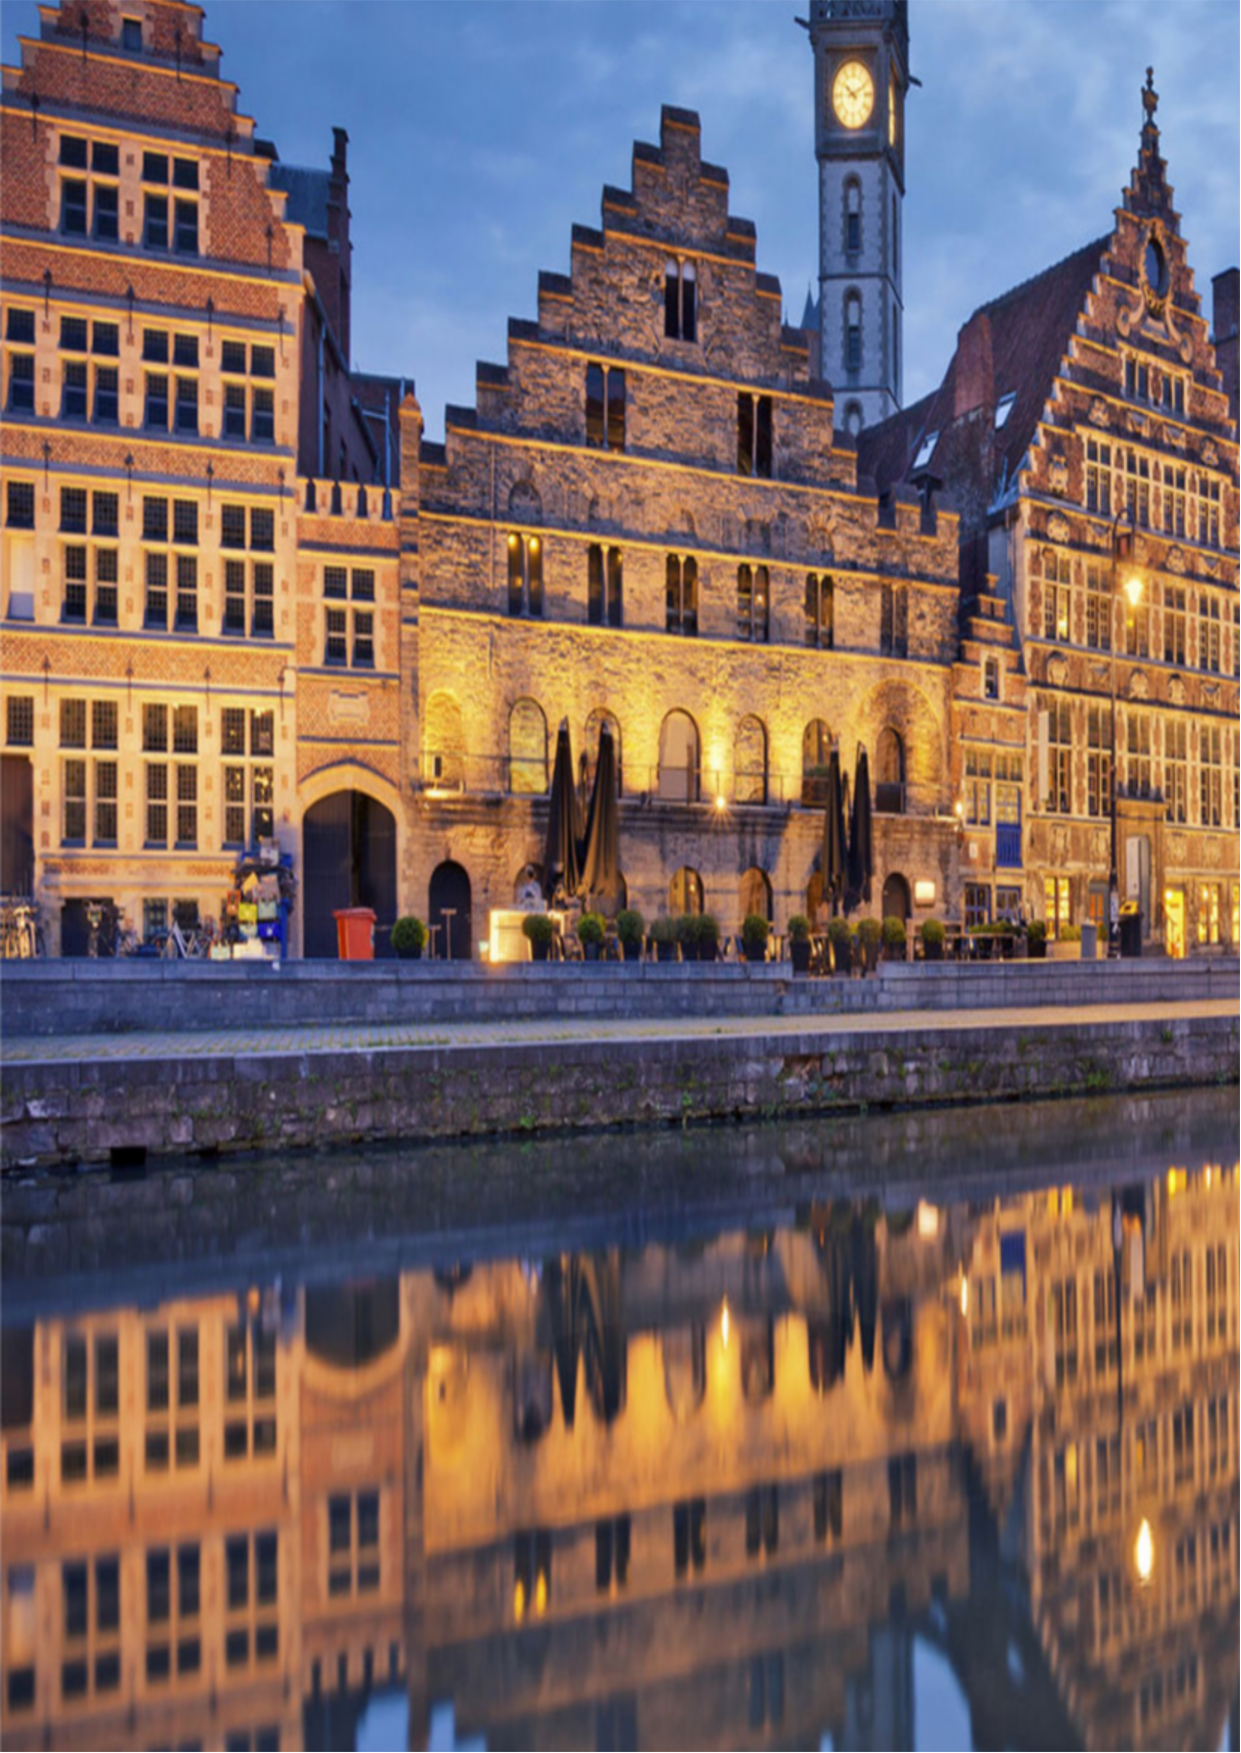
\includepdf{gent_2.pdf}


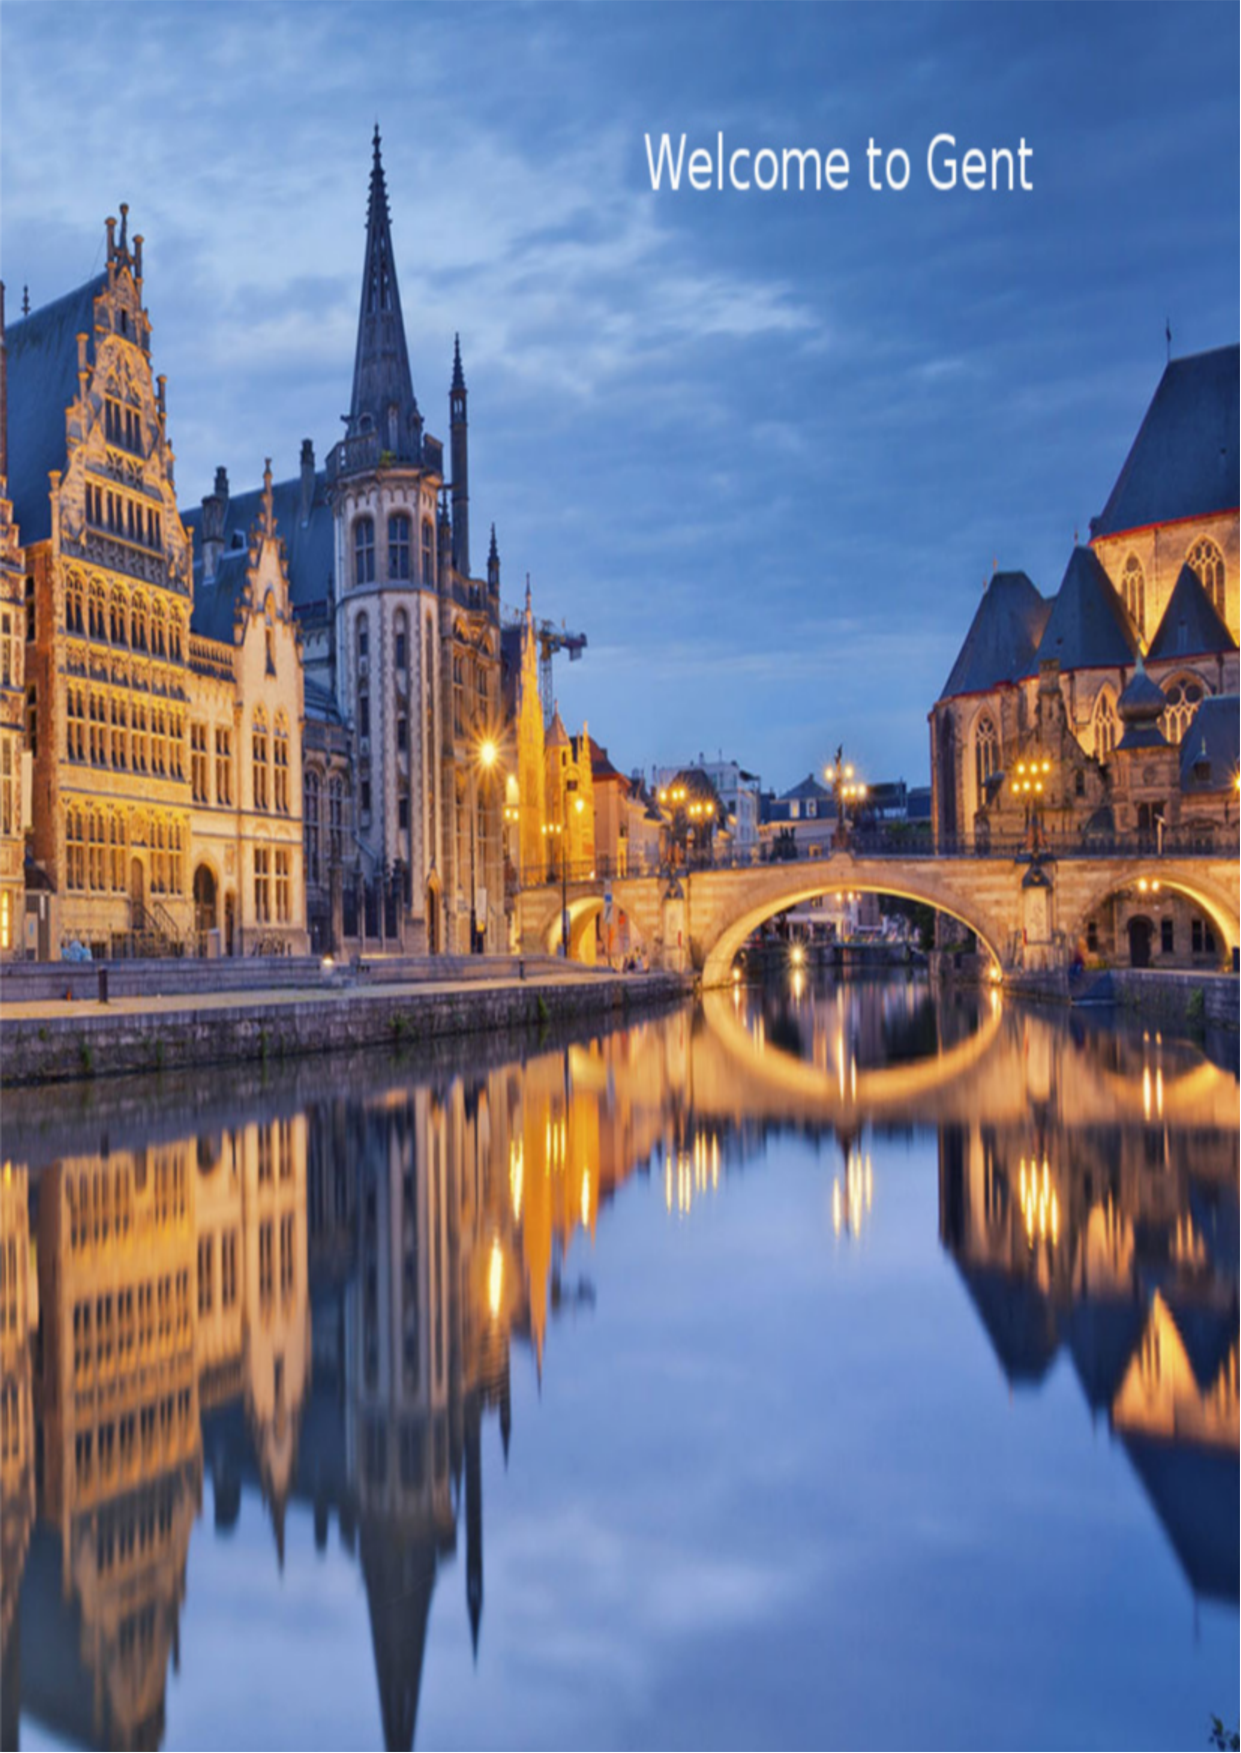
\includepdf{gent_1.pdf}


\chapter{General introduction}


\section*{Cooperative breeding}

Is life

\newpage

\section*{My aims are}

\begin{itemize}
 \item Solve the big questions
 \item please my supervior
\end{itemize}


\newpage


\chapter{Title of paper 1}

\begin{center}
 DVL and many co-authors
\end{center}

\vfill

\textit{Published in an amazing journal}

\newpage

The paper text can be pasted here

\chapter*{Title of Box A}

\addtocontents{toc}{\protect\TocHeadingBoxA}
\label{boxa-pagenb}
\chapter{Summary and discussion}


We learned so many new things

\pagestyle{empty}

\chapter*{References}
\addcontentsline{toc}{chapter}{References}

% voorwoord met dankwoord en toelating tot bruikleen (ondertekend)
%\input{s-voorwoord}

% overzicht
%\include{s-overzicht}

% abstract
%\addcontentsline{toc}{chapter}{Extended abstract}
%\includepdf[pages=-]{../abstract/abstract.pdf}

%\pagestyle{fancy}
%\renewcommand{\baselinestretch}{1.08} 	% De interlinie afstand wat verkleinen.
%\small\normalsize                       % Nodig om de baselinestretch goed te krijgen.
%\addcontentsline{toc}{chapter}{Inhoudsopgave}
%\tableofcontents
%\renewcommand{\baselinestretch}{1.2} 	% De interlinie afstand wat vergroten.
%\small\normalsize                       % Nodig om de baselinestretch goed te krijgen.
%\input{s-afkortingen}


%\input{s-inleiding}
%\input{s-werking}
%\input{s-simulatiemodel}
%\chapter{Implementatie van het simulatiemodel}
%\input{s-nsclick}
%\input{s-uitwerking}
%\input{s-resultaten}
%\input{s-besluit}

\appendix
%\input{s-sourcecode}
%\input{s-details}

% De bibliografie en de index
%\bibliography{bibliodatabase}

\backmatter
\listoffigures
\listoftables
%\addcontentsline{toc}{chapter}{Lijst van codefragmenten}
%\lstlistoflistings

% lege pagina (!!)

% kaft



\end{document}
